%\documentclass{article}

\documentclass[12pt,oneside]{article}
\usepackage[a4paper, left=2.5cm, right=2.5cm, top=2.5cm, bottom=1in]{geometry}

\usepackage{amsmath} 
\usepackage{amssymb} 
\usepackage{amstext}
\usepackage{amsthm}

\usepackage{graphicx}
\usepackage{xcolor}

% for bibliography:
\usepackage{comment} 
%\usepackage[ backend=biber, style=chicago ]{biblatex}
\usepackage[
backend=biber,
style=numeric,
]{biblatex}
\DeclareNameAlias{default}{last-first}

\addbibresource{references.bib}
% see:
% https://www.sharelatex.com/learn/Bibliography_management_in_LaTeX#The_bibliography_file

\usepackage[export]{adjustbox}
%\usepackage{tikz}
%\usetikzlibrary{arrows}
%\usetikzlibrary{scopes}
%\usetikzlibrary{babel}

% For cross references 
%\usepackage{hyperref} 
\usepackage[colorlinks = true]{hyperref}
\usepackage[catalan]{varioref}
%\usepackage{cleveref}
%hyperref configuration so that it doesn't contrast so much colorlinks,
\usepackage{xcolor} 
\hypersetup{ 
   linkcolor={black},
   citecolor={black}, 
   %linkcolor={red!50!black},
   %citecolor={blue!50!black}, 
   urlcolor={blue!80!black} }

% Custom Math operators (functions not in italic in math mode):
\DeclareMathOperator{\arcsec}{arcsec} 
\DeclareMathOperator{\arccot}{arccot}
\DeclareMathOperator{\arccsc}{arccsc} 
\DeclareMathOperator{\cis}{cis}

\usepackage[catalan]{babel} %Names in spanish
\usepackage[utf8]{inputenc} %Use unicode
\usepackage[T1]{fontenc}
\usepackage{csquotes} %For bibliography quotations
\DeclareQuoteAlias{spanish}{catalan}

\usepackage{array} 
\usepackage{float}  %Force tables and images position (H and H!)
\usepackage{wrapfig} %Wrap images like in HTML
\usepackage{minted} %For code blocks
\usepackage{color}  %Custom colors for syntax highlight in listings

\usepackage{tabularx,colortbl, booktabs} %Better tables
%\usepackage[alsoload=hep]{siunitx} %Better tables and SI units and uncertainties
\usepackage{longtable}
%\sisetup{separate-uncertainty=true}
%\sisetup{locale = FR} %commas and so on for spanish
%\sisetup{
  %per-mode=fraction,
  %fraction-function=\nicefrac
%}
\usepackage{multirow}
\usepackage{multicol}
\usepackage{makecell}%Slit cell in lines and more formating options inside table

\usepackage{datetime} %To customize date

\newdateformat{monthyeardate}{%
    \monthname[\THEMONTH], \THEYEAR}
%Now \monthyeardate\today gives the date without the day

%\usepackage[framemethod=tikz]{mdframed} 
\usepackage{nicefrac} %nice fractions in one line

%Subfigures
\usepackage{subcaption} 
\usepackage{relsize} %Bigger math with mathlarger{___}

\usepackage[bottom]{footmisc} %footnote at the bottom

%\renewcommand{\figurename}{Fig.} \renewcommand{\tablename}{Tabla}
%tabla-es in babel better

% Add command before appendix session for page numbering: A-1
\newcommand{\appendixpagenumbering}{
    \break
    \pagenumbering{arabic}
    \renewcommand{\thepage}{\thesection-\arabic{page}}
}

\newcommand{\whitepage}{
    \clearpage\thispagestyle{empty}\addtocounter{page}{-1} \newpage \clearpage
}

\setminted{
frame=lines,
framesep=2mm,
baselinestretch=0.2,
fontsize=\footnotesize,
linenos
}

%\addbibresource{Projecte_A.bib}
%\usepackage{graphicx}

\title{Projecte A - Grafs}
\author{
Aleix Boné Ribó\\
Alex Herrero Pons\\
Alex González Godoy\\
Albert Mercadé Plasencia\\
}
\date{Setembre 2019}

\begin{document}

\thispagestyle{empty}
\clearpage
\setcounter{page}{-1}

\begin{titlepage}
{
    \centering
    \null
    \vfill
    {\Large Projecte d'Algorísmia\par}
    \vspace{2em}
    {\Huge \bfseries 
    Transició de fase i components connexes en grafs aleatoris
    \par}
    \vspace{2em}
    {\large \scshape 
    Grau A \qquad Tardor Curs 2019-2020
    \par}
    \vfill
\begin{center}
    
\end{center}
    \vspace{3cm}

    \vfill
    {\raggedleft \large
Aleix Boné Ribó\\
Alex Herrero Pons\\
Alex González Godoy\\
Albert Mercadé Plasencia\\
        \par}
}
\end{titlepage}

\pagebreak
\pagenumbering{Roman} 

\tableofcontents
\pagebreak
\pagenumbering{arabic} 

\section{Introducció}
%\begin{abstract}

En aquest projecte teníem com a objectiu la investigació de les transicions de fase en algunes propietats dels models de grafs aleatoris Random Binomial Graph (BRG) i Random Geometric Graph (RGG). La connectivitat d'aquests models de grafs és la primera propietat que se'ns demanava explorar, a més, també se'ns requeria indagar sobre la mida esperada de la component connexa més gran al graf. En quant a les propietats extres que nosaltres em escollit per ampliar la nostra investigació, ens hem decantat per:

\begin{itemize}
    \item Existència de camins i cicles Eulerians.
    \item Existència de cicles.
\end{itemize}

%\end{abstract}




\section{Implementació de la classe \texttt{Graph}}
Per representar els grafs hem implementat una classe \texttt{Graph}\footnote{Implementat a src/graph.cpp} que utilitza llistes d'adjacències donat que són més barates en memòria i la implementació d'un \texttt{Breadth First Search (BFS)} menys costosa en comparació amb les matrius d'adjacència.

\begin{listing}
\inputminted{cpp}{src/graph.h}
\caption{Graph.h}
\end{listing}

Dins d'aquesta classe hem implementat la constructora, que inicialitza la llista d'adjacència, i també els següents mètodes:
\begin{itemize}
    \item\texttt{addUndirectedEdge}: donats els identificadors de dos vèrtexs a i b, crea una aresta no dirigida entre ells.
    \item\texttt{addDirectedEdge}: donats els identificadors de dos vèrtexs crea una aresta dirigida entre ells.
    \item\texttt{hasCycles}: retorna un booleà que indica si el graf te cicles. Està implementat utilitzant el mètode \texttt{BFS}.
    \item\texttt{EulerianCycleAndEulerianPath}: expliquem més endavant la seva utilitat e implementació.
    \item\texttt{ConnectedComponents}: expliquem més endavant la seva utilitat e implementació.
    \item\texttt{isConnected}: retorna un booleà que indica si el graf és connex. Està implementat amb un \texttt{BFS}.
    \item\texttt{neighbours}: retorna una llista que conté els veïns del vèrtex.
    \item\texttt{print}: imprimeix per pantalla la morfologia del graf. Utilitzat sobretot per fer tests i \textit{debugar}.
\end{itemize}

% ahora el hasCycles quizas hay que poner que lo explicamos luego no? Supongo no se si hace falta meter lo de lo explicamos luego en todos o lo metemos en general. Como quede mas limpio 
% jajaja okay yo haria esto:

\section{Generació dels Grafs}
\subsection{Random Binomial Graphs}
Per generar un Random Binomial Graph (BRG) ens hem basat en el model d'Erdős-Rényi \cite{Erdos1960OnGraphs,Erdos1959OnI} que per un graf $G=(V,E)$ diu que

\begin{equation}
    \forall u,v \in V,\quad (u,v) \in E \text{ amb probabilitat } p
\end{equation}

Hem implementat l'algoritme prèviament descrit sota la funció \texttt{BRG}\footnote{Implementada a src/graph\_generator.cpp}. Per cada vèrtex veiem totes les possible arestes i seguint una distribució de Bernoulli amb probabilitat $p$ decidim quines afegim i quines no.

\subsection{Random Geometric Graphs}
En un Random Geometric Graph (RGG)\cite{Diaz2007On} per a tot vèrtex $v \in V$ se li assigna unes coordenades ($x_v, y_v$) aleatòries entre 0.0 i 1.0 i les arestes entre dos vèrtex s'afageixen si

\begin{align}
    \forall u,v \in V,\quad (u,v) \in E \Longleftrightarrow \text{dist}(u,v) &\leq r \\
    \text{dist}(u,v) &= \sqrt{\left(x_v - x_u\right)^2 + \left(y_v - y_u\right)^2}
\end{align}

La creació dels RGGs la fem sota la funció \texttt{RGG}\footnote{Implementada a src/graph\_generator.cpp}, on assignem a cada vèrtex unes coordenades aleatòries amb una \texttt{uniform\_real\_distribution}. Després per cada vèrtex iterem la resta i afegim una aresta quan la distància entre els dos vèrtex és menor o igual que el radi \textit{r}.

\section{Comput de dades i generació de gràfiques}

\subsection{Càlcul Adaptatiu}

Al fer les primeres gràfiques ens vam adonar que la gran majoria de punts eren o bé 0, o 1 i la zona de transició de fase
era sovint en un interval molt petit. Per tal d'evitar calcular punts innecessaris al fer les gràfiques però tenir una
bona resolució a l'interval en que es produïa la transició de fase van decidir implementar un mètode de \emp{sampling}
adaptatiu. \footnote{Implementat a src/adaptative\_calc.cpp}

El mètode utilitzat consisteix en dividir els valors de 0 a 1 en 11 punts (0, 0.1, 0.2 ...) i calcular per a cada un dels
punts la mitjana de les 500 repeticions. Un cop feta la primera passada, mirem si hi ha dos valors consecutius en que la
diferència es major a $dy$ calculem el valor pel punt entremig dels dos de manera recursiva fins que la diferència 
sigui menor $dy$ o s'arribi al limit de la recursivitat. Aquest mètode permet obtenir gràfiques que mostren la corba de
transició de fase de manera clara sense haver de computar punts innecessaris del gràfic a les zones planes. Ajustant el valor de $dy$ podem decidir la resolució de la gràfica resultant.

Un cop compilat el programa (amb \texttt{make}), la binària \texttt{main} dins de \emph{bin} calcula utilitzant 
el mètode descrit les dades per les diferents propietats que estudiarem. Es crida de la seguent manera:

\begin{verbatim}
./bin/main tipus_graph propietat N repeticions dy
\end{verbatim}

Descripció dels paràmetres:

\begin{itemize}
    \item  \texttt{tipus\_graph} es el tipus de graf aleatori (\texttt{BRG} o \texttt{GRG})
    \item  \texttt{propietat} es la propietat a calcular (cicle, esConnex, eulerianCycle, eulerianPath, midaCompConMax, numCompCon)
    \item  \texttt{N} es la mida del graf
    \item  \texttt{repeticions} es el nombre de repeticions per cada punt (vam utilitzar 500)
    \item  \texttt{dy} es el valor $dy$ descrit anteriorment (vam utilitzar 0.1 o 0.01 en funció del tipus de dada)
\end{itemize}

\subsection{Generació de gràfiques}

Per generar les gràfiques a partir de les dades calculades, utilitzem les llibreries \emph{matplotlib} i 
\emph{numpy} de \emph{Python 3}. El codi utilitzat per generar els gràfics individuals es troba a \emph{plot.py}.
L'\emph{script} de bash \emph{makePlots.sh} automatitza tot el proces de calcul i generació de les gràfiques.
(\texttt{bash makePlots.sh 10 25 50 60 80 100 150})

\section{Experiments}
\subsection{Probabilitat de ser connex}
%Hipotesis:
En aquest primer experiment la nostra hipòtesi és que sí que trobarem una transició de fase en ambdós casos. En el cas del BRG a mesura que augmenta la probabilitat \emph{p} de que existeixin arestes entre els vèrtex té una certa lògica que augmenti també la probabilitat de ser connex. D'altra banda, en el cas del RGG com més gran és \emph{r} més arestes tindrà cada vèrtex i per tant més alta la probabilitat de que el graf sigui connex.


%Código:
\begin{listing}
\inputminted[firstline=83,lastline=122]{cpp}{src/graph.cpp}
\caption{Funció de ConnectedComponents a graph.cpp}
\end{listing}

Per poder comprovar la hipòtesi i saber quantes components connexes (\textit{cc}) té el \texttt{Random Graph} generat, hem escrit la funció ConnectedComponents\footnote{Implementat a src/graph.cpp}, la qual mitjançant l'algoritme de cerca \texttt{BFS} analitza el gràfic en busca de \textit{cc}. Com es veu en el codi, primerament s'inicialitza un vector de booleans per saber quins vèrtexs ja han estat visitats. Començant pel primer vèrtex i amb l'ajuda d'una cua, es recorren els vèrtexs adjacents no visitats encara mentre s'afegeixen a la cua els veïns d'aquests. Durant la cerca, es manté un comptador de \textit{cc} trobades que s'augmenta quan ja s'han visitat tots els vèrtex de la \textit{cc} actual i encara hi ha veïns per visitar. Un cop la cua ja està buida, és a dir, no hi ha més vèrtexs de la \textit{cc} per visitar, es busca el següent vèrtex no visitat per analitzar una nova component. Finalment retorna un \textit{pair} amb la quantitat de \textit{cc} que hi ha i la mida de la major.

%hola aqui explicas lo de "la grandària de la \textit{cc} que s'esta analitzant en aquell moment i la mida de la més gran del gràfic" que esto seria en CC més gran, borralo

%Merca: como?? yo no he escrito esta parte

%Resultados:
\begin{figure}[H]
    \centering
    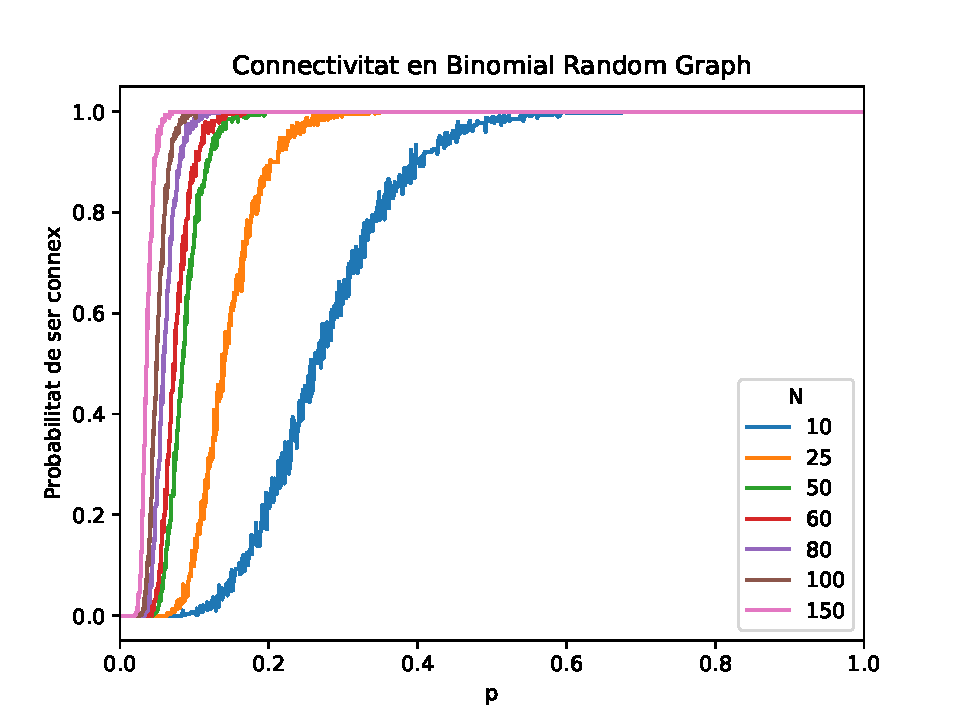
\includegraphics[width=10cm]{plots/BRG_esConnex.pdf}
    \caption{Connectivitat de BRG per diferents valors de \textit{n}}
    \label{fig:connect_04}
\end{figure}

A l'hora d'analitzar els resultats i poder constatar la transició de fase hem plasmat les dades obtingudes en un gràfic on es representa la probabilitat de ser connex de \texttt{BRG} per diferents valors de \textit{n} i per tota possibilitat \textit{p}. A la Figura 1 es pot apreciar una transició de fase més marcada per valors elevats de \emph{N} a probabilitat de \textit{p} propera a 0.05.


\begin{figure}[H]
    \centering
    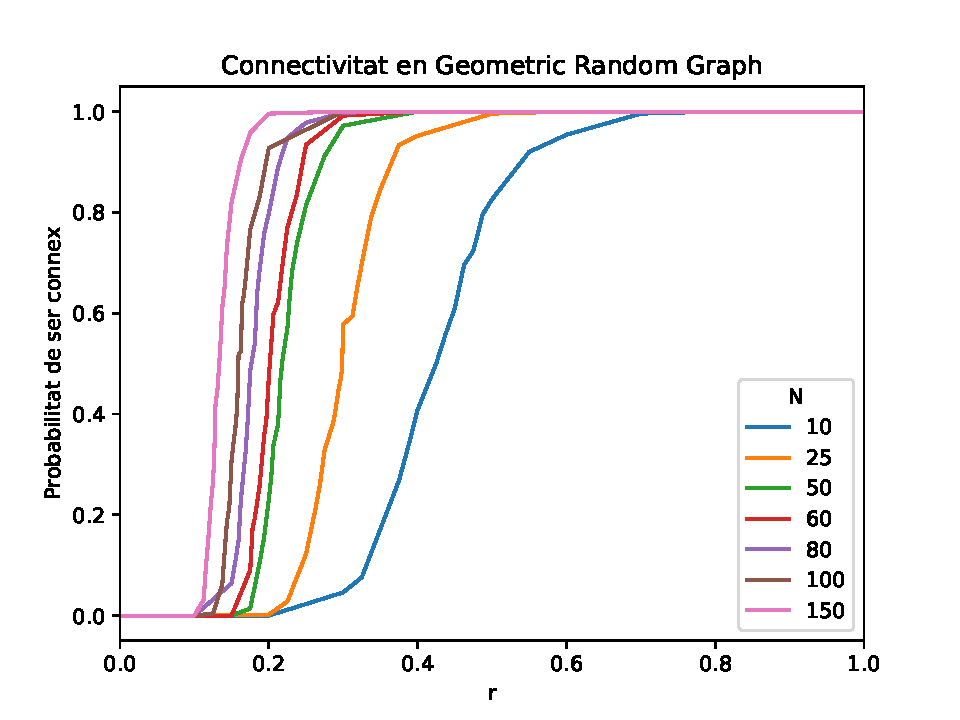
\includegraphics[width=10cm]{plots/GRG_esConnex.pdf}
    \caption{Connectivitat de RGG per diferents valors de \textit{n}}
    \label{fig:connect_04}
\end{figure}

En el cas del \texttt{RGG}, com es pot veure a la Figura 2, representem la probabilitat de que el graf sigui connex respecte el radi \emph{r} per a varis valors de \emph{N}. En aquest cas també apreciem una transició de fase bastant clara que confirma la nostra hipòtesis. A més, semblant al cas del \texttt{BRG}, veiem que la transició és més lenta a mesura que el valor de \emph{N} augmenta. Té sentit que sigui així donat que quants més vèrtex hi han al graf més fàcil és que que hi hagin arestes entre ells connectant-los. En el cas de $N=150$ la transició succeeix molt ràpidament entre els valors de 0.1 i 0.17 de \emph{r}. En canvi per $N=10$ la transició ocorre entre $r=0.25$ i $r=0.6$.


\subsection{Mida esperada CC més gran}
%Hipotesis:
Per aquest experiment, pels mateixos motius que la connectivitat i ja havent confirmat que era l'existència de la transició, vam pensar que seria coherent que la mida esperada de la CC més gran també tingués transició de fase, tant en BRG com en RGG.

%Código: (el mismo que Probabilitat de ser connex)
El codi que hem utilitzat en aquest cas ha sigut el mateix que per la probabilitat de ser connex mostrat més amunt en el Listing 2, però hem afegit dues variables (\textit{size}, \textit{max}) per tal de comprovar quina component és la més gran.

%Resultados:
\begin{figure}[H]
    \centering
    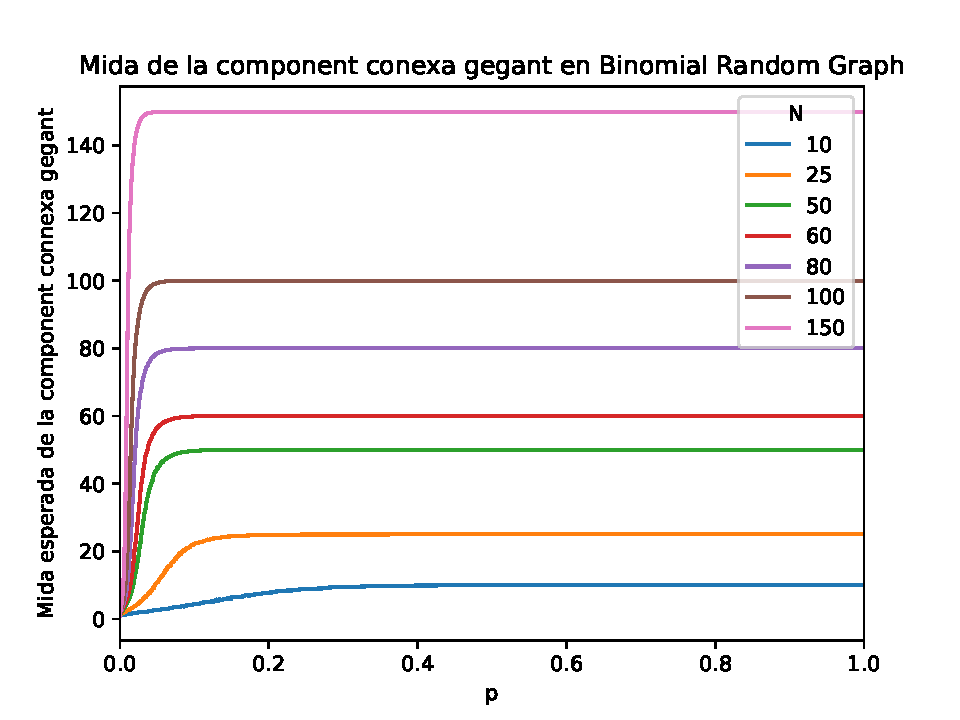
\includegraphics[width=10cm]{plots/BRG_midaCompConMax.pdf}
    \caption{Mida esperada de la CC més gran de BRG per diferents valors de \textit{n}}
    \label{fig:connect_04}
\end{figure}

Amb els resultats obtinguts es pot veure clarament una transició de fase propera a \textit{p=}0.05, la qual era en certa mida previsible després dels resultats de la connectivitat de \texttt{BRG} per a diferents valors de \textit{n}, ja que la mida d'una component connexa gegant és inversament proporcional a la quantitat de components connexes. %AQUI NS SI ME ACABO DE FLIPAR. pues si, pero tiene sentido

\begin{figure}[H]
    \centering
    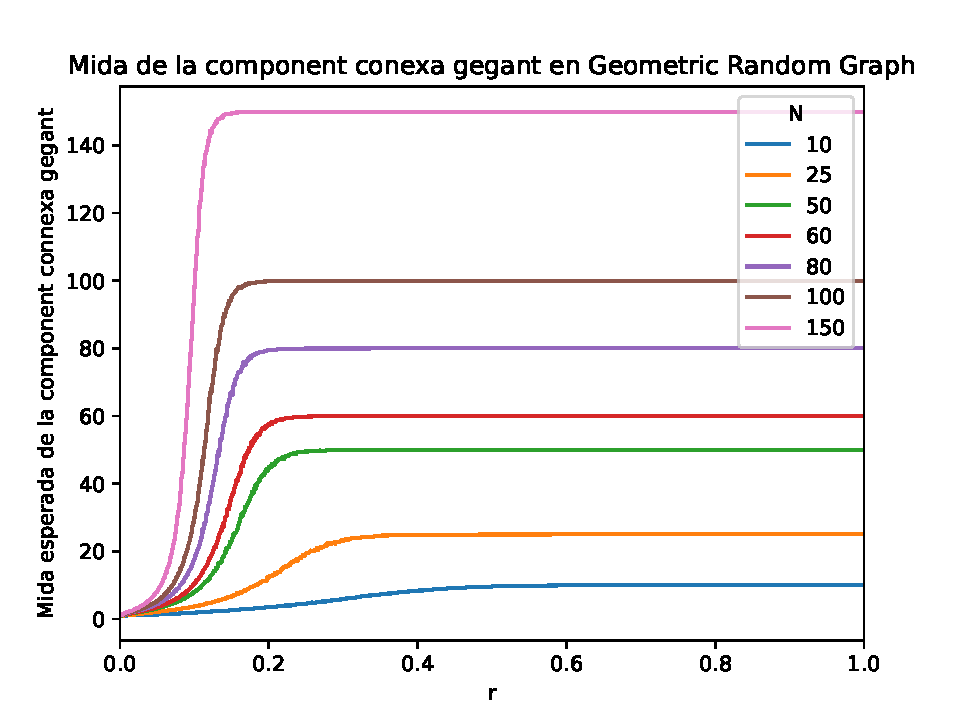
\includegraphics[width=10cm]{plots/GRG_midaCompConMax.pdf}
    \caption{Mida esperada de la CC més gran de RGG per diferents valors de \textit{n}}
    \label{fig:connect_04}
\end{figure}

En el cas de \texttt{RGG} els resultats representats ens ajuden a veure una transició de fase ben marcada a \textit{p=0.1} la qual correspon a la obtinguda en el anàlisi de la connectivitat de \texttt{RGG} per diferents valors de \textit{n}. Com esmentat anteriorment, aquests resultats venen justificats pel fet de la proporcionalitat inversa entre el nombre de \textit{cc} i la mida de la component connexa gegant. %Igual que antes, ns si me he flipado.

\subsection{Camí i cicle Eulerià}
%Hipotesis:
En aquest tercer experiment hem volgut comprobar si la probabilitat de tenir un camí o un cicle Eulerià tindría transició de fase. Vam escollir aquesta propietat perque ens semblava més arbitrària i que per tant no tindría transició de fase.

%Código:
\begin{listing}
\inputminted[firstline=8,lastline=8]{cpp}{src/graph.h}
\inputminted[firstline=60,lastline=81]{cpp}{src/graph.cpp}
\caption{Funció de EulerianCycleAndEulerianPath en graph.cpp}
\end{listing}

Per determinar si un graf té un cicle Eulerià o un camí Eulerià hem creat la funció \textttt{EulerianCycleAndEulerianPath}\footnote{Implementada a src/graph.cpp}. Primerament utilitzant la funció \textttt{ConnectedComponents} comprova que tots el vèrtex amb grau \textit{g > 0} pertanyen a una única Component Connexa, si és el cas simplement mirant el nombre de vèrtexs amb grau imparell podem classificar si tenen un camí (dos vèrtexs imparells) o si tenen un cicle, i per tant també un camí (cap vèrtex imparell).

%Resultados:
\begin{figure}[H]
    \centering
    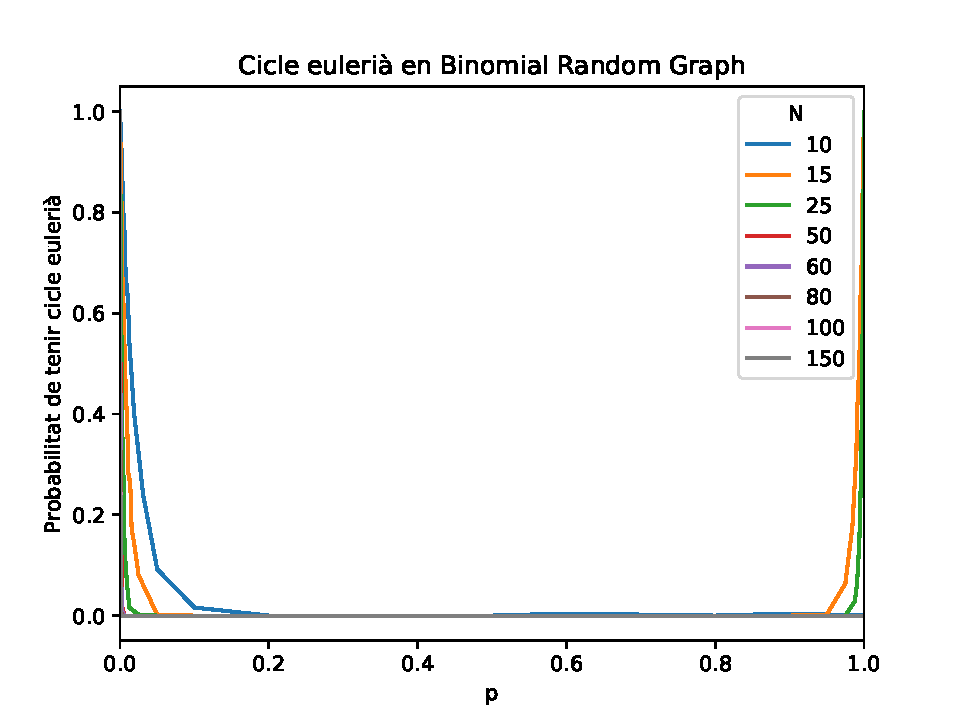
\includegraphics[width=10cm]{plots/BRG_eulerianCycle.pdf}
    \caption{Eulerian Cycle de BRG per diferents valors de \textit{n}}
    \label{fig:connect_04}
\end{figure}

Com es pot veure a la Figura 5, es podria considerar l'existència d'una transició de fase per valors de \textit{p} propers a 0 ja que en aquell moment tot vèrtex amb $g=0$ es considera cicle Eulerià. Però la probabilitat de contenir un cicle Eulerià baixa dràsticament ja que s'han de donar les condicions que hi hagi un cicle i que a més aquest sigui Eulerià. Finalment, es pot veure que amb valors de \textit{p} pròxims a 1, la probabilitat que un gràfic $N=25$, contingui un cicle Eulerià creix fins a 1 un altre cop. Això es deu a que tenir $p=1$ obtens un gràfic complet el qual, si el nombre de vèrtexs és imparell, tindrà un cicle Eulerià.

\begin{figure}[H]
  i  \centering
    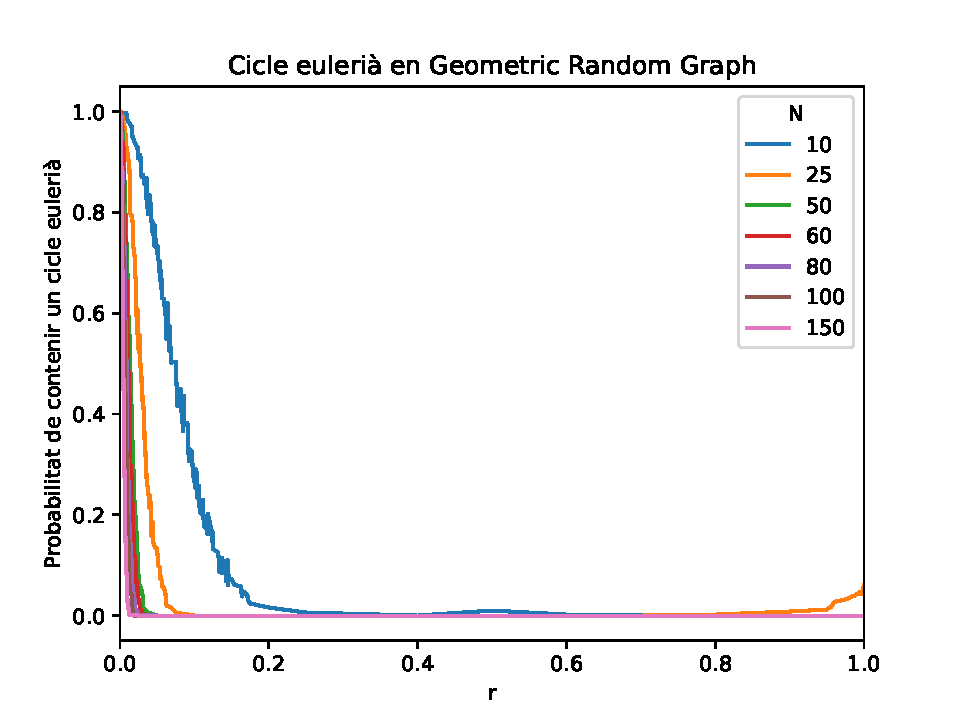
\includegraphics[width=10cm]{plots/GRG_eulerianCycle.pdf}
    \caption{Eulerian Cycle de RGG per diferents valors de \textit{n}}
    \label{fig:connect_04}
\end{figure}

En el cas de \texttt{RGG}, la transició de fase està present per a valors de \textit{p} propers a 0, però en aquest cas, a diferència del \texttt{BRG}, no està tant marcada quan el nombre de vèrtexs és petit. Igual que en el cas de \texttt{BRG}, els vèrtexs amb grau 0 es consideren cicles Eulerians. De nou, amb valors molt elevats de \textit{p} i amb nombre imparell de vèrtexs es pot veure que la probabilitat que contingui un cicle Eulerà torna a créixer. %esto esta bien? a ver, no lo veo mal

\begin{figure}[H]
    \centering
    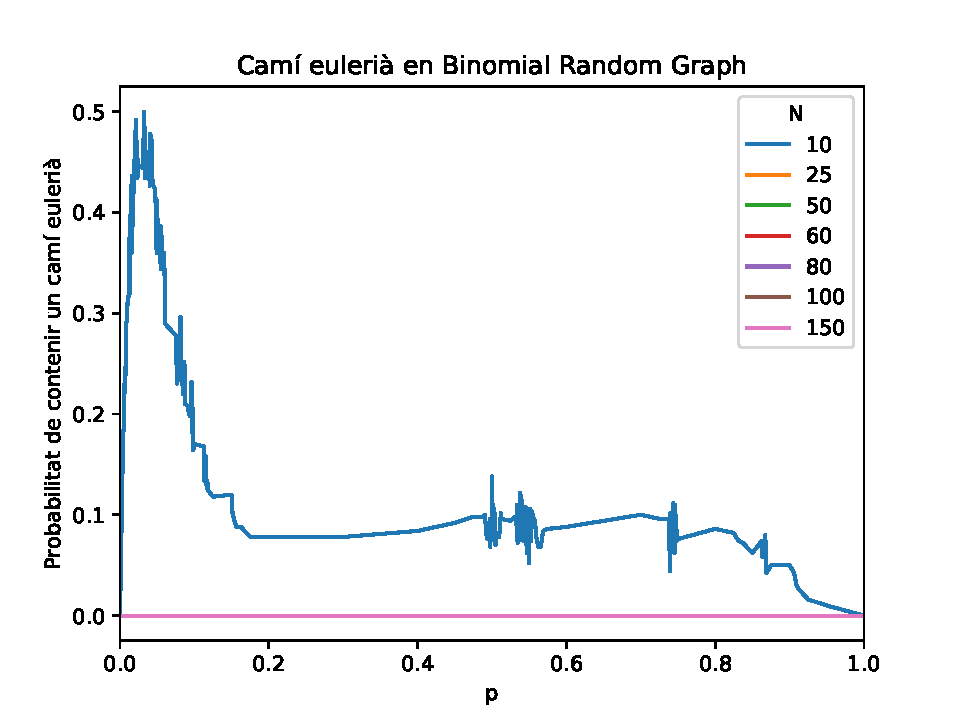
\includegraphics[width=10cm]{plots/BRG_eulerianPath.pdf}
    \caption{Eulerian Path de BRG per diferents valors de \textit{n}}
    \label{fig:connect_04}
\end{figure}

AQUI FALTA COMENTAR LOS RESULTADOS

\begin{figure}[H]
    \centering
    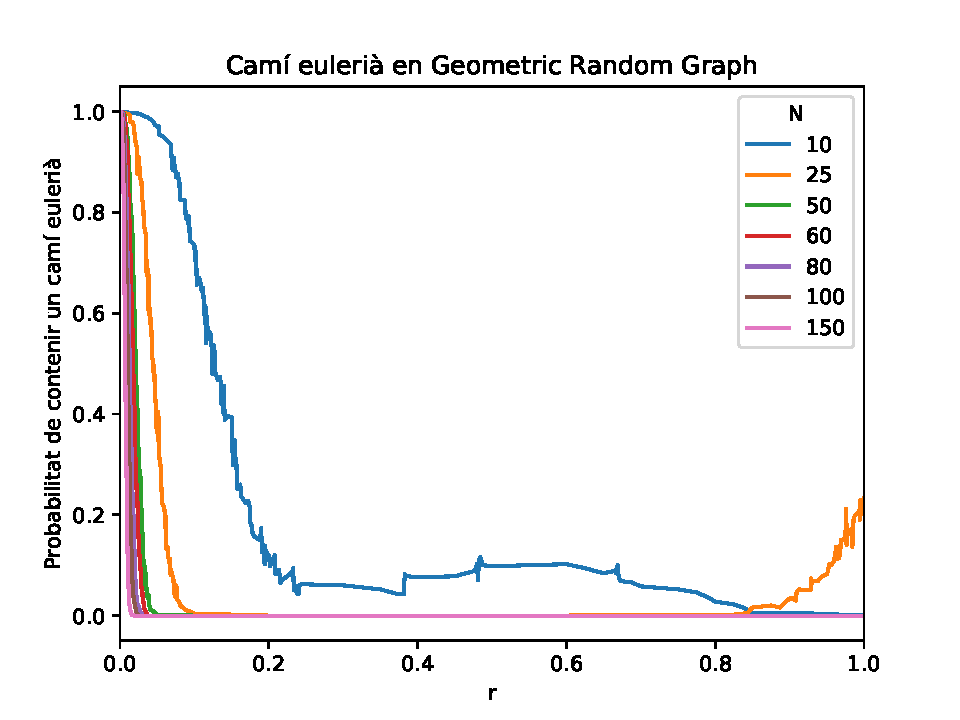
\includegraphics[width=10cm]{plots/GRG_eulerianPath.pdf}
    \caption{Eulerian Path de RGG per diferents valors de \textit{n}}
    \label{fig:connect_04}
\end{figure}

AQUI FALTA COMENTAR LOS RESULTADOS

\subsection{Probabilitat de contenir un cicle}
%Hipotesis:
L'últim experiment que hem realitzat és veure si la probabilitat de que un graf contingui un cicle té transició de fase o no. Abans de realitzar l'experiment, havent vist que el cicle Eulerià si que tenia transició de fase vam anticipar que en aquest cas també en tindria i més remarcada.

%Código:
\begin{listing}
\inputminted[firstline=27,lastline=57]{cpp}{src/graph.cpp}
\caption{Funció de hasCylces Funció TreeAndForest en graph.cpp}
\end{listing}

Per comprovar si el graf conté algún cicle hem creat la funció \textit{hasCycles} que recorre el graf amb un \texttt{BFS} i si en la mateixa component conexa torna a visitar un mateix vértex retorna que ha trobat un cicle.

%Resultados:
\begin{figure}[H]
    \centering
    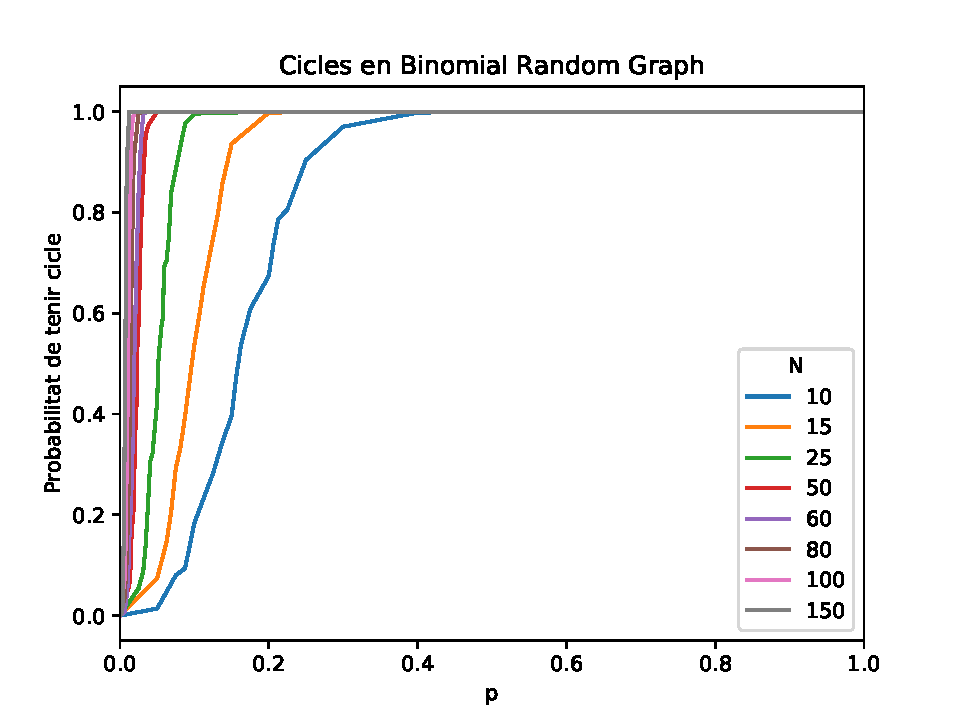
\includegraphics[width=10cm]{plots/BRG_cicle.pdf}
    \caption{Probabilitat de tenir un cicle de BRG per diferents valors de \textit{n}}
    \label{fig:connect_04}
\end{figure}

AQUI FALTA COMENTAR LOS RESULTADOS

\begin{figure}[H]
    \centering
    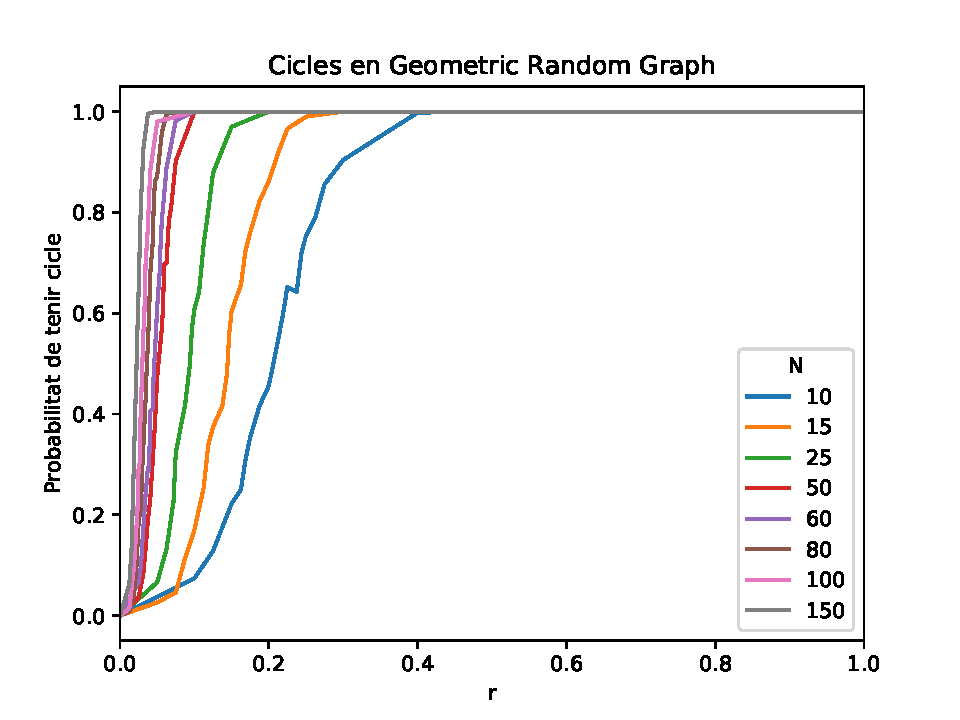
\includegraphics[width=10cm]{plots/GRG_cicle.pdf}
    \caption{Probabilitat de tenir un cicle de RGG per diferents valors de \textit{n}}
    \label{fig:connect_04}
\end{figure}

AQUI FALTA COMENTAR LOS RESULTADOS

\section{Possibles futurs experiments}
Com a possibles experiments que finalment no hem volgut exposar havíem fet, aprofitant la probabilitat de si un graf conté un cicle, la probabilitat de que el graf sigués un arbre o un bosc per separat, però veient els resultats no tenía gaire sentit. També havíem pensat en veure si hi ha transició de fase en la probabilitat de que hi hagi un camí o cicle Hamiltonià. A més també havíem considerat indagar la existència de transició de fase de que els grafs siguin bipartits.

\section{Conclusions}

\pagebreak

\printbibliography

\end{document}
